\documentclass[11pt,a4paper]{article}
\usepackage[margin=25mm,headheight=15pt]{geometry}
\usepackage[T1]{fontenc}
\usepackage[utf8]{inputenc}
\usepackage{libertinus}
\usepackage{amsmath,amssymb,amsthm,mathtools}
\usepackage{microtype,booktabs,array,longtable,graphicx}
\usepackage{xcolor,fancyhdr,titlesec,enumitem,xurl}
\usepackage{aliascnt}
\usepackage{hyperref}
\usepackage[nameinlink,noabbrev]{cleveref}
\definecolor{ink}{RGB}{24,49,70}
\definecolor{muted}{RGB}{82,88,94}
\hypersetup{colorlinks=true,linkcolor=ink,citecolor=ink,urlcolor=ink,
 pdftitle={Periodic Anchors and Exact Mixed-Moment Phase Diagrams},
 pdfauthor={Research draft prepared with ChatGPT for Vladimir Reshetnikov},
 pdfsubject={Digital products, singular coboundaries, pressure, periodic equilibrium selection and critical moments}}
\titleformat{\section}{\Large\bfseries\color{ink}}{\thesection}{.65em}{}
\titleformat{\subsection}{\large\bfseries}{\thesubsection}{.65em}{}
\pagestyle{fancy}\fancyhf{}
\fancyhead[L]{\small Periodic anchors and exact mixed moments}
\fancyhead[R]{\small ProveIt research}
\fancyfoot[C]{\thepage}
\setlength{\emergencystretch}{3em}
\setlength{\parskip}{.22em}
\setlist{itemsep=.25em,topsep=.4em}
\allowdisplaybreaks
\numberwithin{equation}{section}
\newtheorem{theorem}{Theorem}[section]
\newaliascnt{lemma}{theorem}
\newtheorem{lemma}[lemma]{Lemma}\aliascntresetthe{lemma}
\newaliascnt{proposition}{theorem}
\newtheorem{proposition}[proposition]{Proposition}\aliascntresetthe{proposition}
\newaliascnt{corollary}{theorem}
\newtheorem{corollary}[corollary]{Corollary}\aliascntresetthe{corollary}
\theoremstyle{definition}
\newaliascnt{definition}{theorem}
\newtheorem{definition}[definition]{Definition}\aliascntresetthe{definition}
\newtheorem{question}{Research question}
\theoremstyle{remark}
\newaliascnt{remark}{theorem}
\newtheorem{remark}[remark]{Remark}\aliascntresetthe{remark}
\newcommand{\TT}{\mathbb T}
\newcommand{\RR}{\mathbb R}
\newcommand{\CC}{\mathbb C}
\newcommand{\NN}{\mathbb N}
\newcommand{\ZZ}{\mathbb Z}
\newcommand{\dd}{\,\mathrm d}
\newcommand{\ee}{\mathrm e}
\newcommand{\Leb}{\mathrm{Leb}}
\newcommand{\cM}{\mathcal M}
\newcommand{\cE}{\mathcal E}
\newcommand{\cO}{\mathcal O}
\newcommand{\cD}{\mathcal D}
\newcommand{\PP}{\mathcal P}
\newcommand{\supp}{\operatorname{supp}}
\newcommand{\conv}{\operatorname{conv}}
\newcommand{\lcm}{\operatorname{lcm}}
\newcommand{\norm}[1]{\left\lVert #1\right\rVert}
\newcommand{\abs}[1]{\left|#1\right|}
\newcommand{\code}[1]{\texttt{\detokenize{#1}}}

\begin{document}
\hypersetup{pageanchor=false}
\begin{titlepage}
\thispagestyle{empty}\setlength{\parindent}{0pt}
{\small\sffamily\color{ink} PROVEIT\quad /\quad ANALYSIS AND DYNAMICAL SYSTEMS}\par
\vspace{12mm}
{\Huge\bfseries\color{ink} Periodic Anchors and\\[3mm]
Exact Mixed-Moment\\[3mm] Phase Diagrams\par}
\vspace{7mm}
{\Large Singular coboundaries, explicit freezing surfaces,\\[2mm]
and arithmetic leading amplitudes\par}
\vspace{8mm}
{\large Research draft prepared for Vladimir Reshetnikov\par}
{Prepared with ChatGPT\quad\textbullet\quad 30 September 2026\par}
\vspace{5mm}\hrule\vspace{3mm}
\begin{abstract}
We identify a globally solvable class of genuinely mixed digital products.
For the map $T_bx=bx\pmod1$, place phase shifts on finitely many complete
periodic orbits $\cO_i$, with a common positive exponent $a_i$ on each orbit.
The product of normalized digital masks is a singular coboundary.
It changes the energy of every invariant measure avoiding the selected
orbits by the same amount, but gives each selected orbit an explicit
additional reward. For an arbitrary continuous nonnegative background
weight $v$ of finite pressure, we prove
\[
 \PP_b\!\left(v\prod_i\prod_{p\in\cO_i}m_b(\cdot-p)^{a_i}\right)
 =-D\log b+\max\left\{\PP_b(v),\ \max_i(Q_i(v)+a_i\log b)\right\},
\]
where $D=\sum_i a_i|\cO_i|$ and $Q_i(v)$ is the orbit average of $\log v$.
For a squared shifted digital background, Parseval gives $\PP_b(v)=0$
at every phase. A subharmonic sampling estimate converts this formula
into explicit mixed-moment growth exponents for arbitrary positive real
anchor exponents. Without a background we also determine leading
constants, logarithmic critical terms, and uniform critical windows.
An exactly evaluated seventh-root example has leading amplitudes $3,4,4$
according to the depth modulo three. We construct prescribed finite
polyhedral pressure diagrams and extend orbit selection to nonlinear
expanding circle maps. Full proofs, exact-arithmetic checks, numerical
diagnostics, and a research agenda are included.
\end{abstract}
\vfill
{\small\color{muted} Status: unrefereed mathematical research draft; not Lean-verified.
The results are proved derivations, not independently established claims
of worldwide priority. Numerical diagnostics do not replace the proofs.}
\end{titlepage}
\hypersetup{pageanchor=true}
\begingroup\small\setlength{\parskip}{0pt}\tableofcontents\endgroup
\newpage

\section{Research target, contribution, and limits}
\label{sec:intro}
\subsection{Why mixed digital products are a useful next target}
The Fabius--Rvachev--Thue--Morse part of ProveIt contains finite-product
identities, moment computations, and recent manuscripts on integer,
fractional, critical, and subcritical digital-product pressure
\cite{Repo,RepoIndex}. The single-phase critical law is already treated
there. This article therefore does not claim to discover that law or to
fill an endpoint gap already addressed by later drafts. It changes the
problem: several phase-shifted digital products are multiplied before
taking a moment.

The recent primary literature relates generalized Thue--Morse Riesz
products to thermodynamic pressure and fractal spectra \cite{GKS}.
Continuity in the location of a logarithmic singularity, and the problem
of stronger positive-order phase regularity, are studied in \cite{GLS}.
Our results concern an exactly structured mixed family, not a general
solution of that phase-regularity problem.

For a single atomic mask, telescoping is familiar. The additional
observation is that telescoping survives for an entire periodic orbit of
phase shifts, and for any finite collection of such orbits. The singularity
then distinguishes measures supported on the selected orbits from all
other invariant measures. This yields a finite maximum of explicit
pressure branches rather than a perturbative approximation to an unknown
spectral radius.

The principal payoff is the exact mixed-moment exponent in
\cref{thm:mixed}. It holds globally in the background phase, in every
integer base, and for arbitrary positive real anchor exponents. The
orbit-balance condition is essential. We make no claim to evaluate
arbitrary unrelated phase tuples.

\subsection{What is proved, and what is inherited}
A one-sided integrability lemma makes singular coboundary cancellation
legitimate. A variational principle with zero weights turns the resulting
energy identity into an exact pressure formula and a classification of
its equilibrium faces. A sampling estimate for products of absolute
powers of polynomials identifies the corresponding moment exponent.
The thermodynamic inputs inherited from classical theory are the
continuous-potential variational principle and the usual entropy facts
for an expanding map \cite{Walters}; the extension at zeros is proved here.

No fractional-cusp, critical-cusp, or spectral-perturbation theorem from
an unreviewed repository draft is needed in this chain. The exact
finite-product normalization is also derived directly. Future revisions
of the neighboring pressure manuscripts therefore do not affect these
proofs.

For orbit-balanced products without a background, we determine
subcritical constants, critical logarithms, supercritical residue-class
amplitudes, and a multivariate critical crossover. An explicit
three-phase example is evaluated exactly at every depth, not merely to
leading order.

\subsection{Provenance and novelty boundary}
The repository index was inspected at the pinned commit
\begin{center}\small\nolinkurl{781594d886f8dc56069221e2b56bd1e94d9c6e5f}.\end{center}
The relevant index is under
\begin{quote}\small
\path{Analysis/FabiusFunction/docs/semi-formalized-research-frontiers/drafts/thue-morse/README.md}.
\end{quote}
It explicitly labels the recent pressure arrivals unreviewed and without
Lean statements. We retain the distinction between mathematical
exposition, numerical evidence, and formal proof.

The finite polyhedral realization result in \cref{sec:realization} is
not a claim that pressure flexibility is new. Kucherenko and Quas prove
much broader realization results for continuous potentials on compact
symbolic systems \cite{KQ}. Our contribution there is a finite explicit
trigonometric construction on a fixed expanding circle map, with chosen
periodic equilibrium measures and logarithmically singular potentials.
The restricted source search did not establish an independent priority
claim for the complete package of formulas below.

\section{Definitions and principal formulas}
\label{sec:definitions}
Fix an integer $b\ge2$, put $B=\log b$, and write
$T=T_b\colon\TT\to\TT$, $Tx=bx\pmod1$, where $\TT=\RR/\ZZ$.
All logarithms are natural unless a base is displayed. Define
\begin{equation}
 d_b(x)=\frac1b\sum_{r=0}^{b-1}\ee^{2\pi i r x},\qquad
 m_b(x)=|d_b(x)|=
 \left|\frac{\sin\pi bx}{b\sin\pi x}\right|.
 \label{eq:mask}
\end{equation}
At integers the quotient has removable value $1$.
Thus $0\le m_b\le1$, and $m_2(x)=|\cos\pi x|$.

\subsection{Pressure for a weight which may vanish}
For a continuous $w\colon\TT\to[0,\infty)$ set
\begin{align}
 w^{(n)}(x)&=\prod_{j=0}^{n-1}w(T^jx), & N&=b^n,\\
 Z_n(w)&=\sum_{k=0}^{N-1}
       \sup_{x\in[k/N,(k+1)/N]}w^{(n)}(x),
 &\PP_b(w)&=\lim_{n\to\infty}\frac1n\log Z_n(w).
 \label{eq:pressure}
\end{align}
The limit and its variational meaning are proved in
\cref{sec:variational}. We write $\PP_b(w)$ rather than $P(\log w)$
to keep zeros visible. Thus $\PP_b(cw)=\log c+\PP_b(w)$ for $c>0$
and $\PP_b(1)=B$. An equilibrium measure maximizes
$h_\mu(T)+\int\log w\dd\mu$, with $\log0=-\infty$.

There is no factor $1/b$ in the associated transfer operator
$L_w f(x)=\sum_{Ty=x}w(y)f(y)$. The exponent of a Lebesgue moment is
$\PP_b(w)-B$, not $\PP_b(w)$, whenever the moment-pressure conversion
below applies.

\subsection{Periodic anchors}
Let $\cO_1,\ldots,\cO_m$ be pairwise disjoint periodic orbits of $T$,
with lengths $r_i$. Give every point of $\cO_i$ the same exponent
$a_i>0$. Put
\begin{align}
 E&=\bigcup_i\cO_i, & D&=\sum_i r_i a_i,\\
 A_{\boldsymbol a}(x)&=\prod_i\prod_{p\in\cO_i}m_b(x-p)^{a_i},
 &\Phi_{\boldsymbol a}(x)&=
       \prod_i\prod_{p\in\cO_i}|\sin\pi(x-p)|^{a_i}.
 \label{eq:anchors}
\end{align}
Exponent zero means that the orbit is omitted; no interpretation of
$0^0$ is needed. For a background $v\ge0$ define
\begin{equation}
 Q_i(v)=\frac1{r_i}\sum_{p\in\cO_i}\log v(p).
 \label{eq:orbit-mean}
\end{equation}
If $v$ vanishes at one point of $\cO_i$, then $Q_i(v)=-\infty$.
Let $\delta_i=r_i^{-1}\sum_{p\in\cO_i}\delta_p$.

\begin{theorem}[Exact periodic-anchor pressure]
\label{thm:pressure}
Let $v\colon\TT\to[0,\infty)$ be continuous with
$\PP_b(v)>-\infty$. Then
\begin{equation}
 \boxed{\quad
 \PP_b(vA_{\boldsymbol a})
 =-DB+\max\left\{\PP_b(v),\ \max_i
                   \bigl(Q_i(v)+a_iB\bigr)\right\}.
 \quad}
 \label{eq:main-pressure}
\end{equation}
Write the maximum as $C$. The equilibrium measures of
$vA_{\boldsymbol a}$ are exactly the convex combinations of the following
available measures: all equilibrium measures of $v$ when $C=\PP_b(v)$,
and $\delta_i$ for each $i$ with $Q_i(v)+a_iB=C$.
\end{theorem}
Whenever the background branch wins, all its equilibrium measures give
zero mass to $E$. No uniqueness hypothesis on the background is required.

\begin{corollary}[No background]
\label{cor:no-background-pressure}
For $v=1$,
\begin{equation}
 \PP_b(A_{\boldsymbol a})
 =B\left(\max\{1,a_1,\ldots,a_m\}-D\right).
 \label{eq:pure-pressure}
\end{equation}
If all $a_i<1$, the unique equilibrium measure is Lebesgue measure.
If the largest $a_i>1$, equilibrium measures are exactly the mixtures
of orbit measures with that largest exponent. At a maximum equal to
$1$, Lebesgue measure and precisely the orbits with exponent $1$ coexist.
\end{corollary}
The maximal-entropy measure for $T_b$ is uniquely Lebesgue measure:
the uniform Bernoulli coding has entropy $\log b$, and equality in the
finite-alphabet entropy bound forces independent uniform digits.

\subsection{The mixed digital moment}
Let $s_b(k)$ denote the sum of the base-$b$ digits of $k$, and put
\begin{equation}
 S_{n,c}(x)=\sum_{k=0}^{b^n-1}
         \ee^{2\pi i(kx-cs_b(k))}.
 \label{eq:digital-sum}
\end{equation}
This sign convention gives binary classical Thue--Morse phase $c=1/2$
and Dirichlet-kernel phase $c=0$. For a squared background set
\begin{equation}
 Q_i(c)=\frac2{r_i}\sum_{p\in\cO_i}\log m_b(p-c).
 \label{eq:qi-c}
\end{equation}

\begin{theorem}[Global mixed-moment exponent]
\label{thm:mixed}
For every real phase $c$ and every positive real vector $\boldsymbol a$,
the moment
\begin{equation}
 I_n(\boldsymbol a,c)=\int_0^1|S_{n,c}(x)|^2
        \prod_i\prod_{p\in\cO_i}|S_{n,p}(x)|^{a_i}\dd x
 \label{eq:mixed-moment}
\end{equation}
satisfies, with $N=b^n$,
\begin{equation}
 \boxed{\quad
 \lim_{n\to\infty}\frac{\log I_n(\boldsymbol a,c)}{\log N}
 =1+\max\left\{0,\ \max_i\left(a_i+\frac{Q_i(c)}B\right)\right\}.
 \quad}
 \label{eq:mixed-exponent}
\end{equation}
Branches with $Q_i(c)=-\infty$ are omitted. Equivalently, if the exponent
is $\gamma$, then $I_n=N^{\gamma+o(1)}$.
\end{theorem}
This is not an assertion that $I_n/N^\gamma$ converges. Logarithmic
factors and arithmetic oscillations are not ruled out. Both phenomena
will occur in the family without a background.

\section{Two foundations: zero weights and singular cancellation}
\label{sec:variational}
\subsection{A variational principle which includes zeros}
\begin{lemma}
\label{lem:variational}
For every continuous $w\ge0$, the limit in \cref{eq:pressure} exists in
$[-\infty,\infty)$ and
\begin{equation}
 \PP_b(w)=\sup_{\mu\in\cM_T}
      \left(h_\mu(T)+\int\log w\dd\mu\right),
 \label{eq:vp}
\end{equation}
where $\cM_T$ is the set of invariant Borel probability measures.
If $\PP_b(w)>-\infty$, the supremum is attained.
\end{lemma}
\begin{proof}
Every $(n+k)$-cylinder is specified by an $n$-cylinder and a $k$-cylinder
for its image under $T^n$. Splitting the product at time $n$ gives
$Z_{n+k}(w)\le Z_n(w)Z_k(w)$. Fekete's lemma yields
$\PP_b(w)=\inf_{n\ge1}n^{-1}\log Z_n(w)$. If some $Z_n=0$,
later products vanish and the extended-real interpretation is immediate.

For $\varepsilon>0$, the potential $\log(w+\varepsilon)$ is continuous,
so the ordinary variational principle \cite{Walters} applies. The
$b$-adic coding identifies our partition sum with the full-shift cylinder
sum. The coding is at most two-to-one and adds zero relative entropy;
it preserves the variational value. Thus this application has exactly
our normalization.

For fixed $n$, uniform convergence gives
$Z_n(w+\varepsilon)\to Z_n(w)$. Consequently
\begin{equation}
 \PP_b(w+\varepsilon)\downarrow\PP_b(w).
 \label{eq:pressure-monotone}
\end{equation}
Monotonicity gives one bound; for each fixed $n$ the limiting pressure
is at most $n^{-1}\log Z_n(w)$, giving the other after taking the infimum.

The entropy map is upper semicontinuous for $T_b$, by positive
expansiveness. To justify the singular limit explicitly, choose
equilibrium measures $\mu_j$ for $w+\varepsilon_j$, with
$\varepsilon_j\downarrow0$, and take a weakly convergent subsequence
$\mu_j\to\mu$. For fixed $\delta>0$ and large $j$,
\[
 \PP_b(w+\varepsilon_j)
 \le h_{\mu_j}(T)+\int\log(w+\delta)\dd\mu_j.
\]
Upper semicontinuity of entropy and continuity of the second term give
\[
 \PP_b(w)\le h_\mu(T)+\int\log(w+\delta)\dd\mu.
\]
Let $\delta\downarrow0$, using monotone convergence after subtracting
an upper bound. Conversely, apply the continuous variational principle
to any invariant measure and take the same limit. This proves
\cref{eq:vp}; when the value is finite the limiting measure attains it.
If the value is $-\infty$, the converse bound already forces every
variational value to be $-\infty$.
\end{proof}

\subsection{Why infinite logarithmic integrals cannot simply be canceled}
A formal identity $g=u\circ T-u$ does not permit subtraction of two
infinite integrals. The following lemma is the precise substitute.
\begin{lemma}[One-sided stationary cancellation]
\label{lem:cancellation}
Suppose $T$ preserves a probability measure $\mu$ and
$U\colon X\to[0,\infty)$ is finite almost everywhere. If
$U-U\circ T$ is bounded above, then it is integrable and
\begin{equation}
 \int(U-U\circ T)\dd\mu=0.
 \label{eq:cancellation}
\end{equation}
The same holds with ``bounded below'' in place of ``bounded above.''
\end{lemma}
\begin{proof}
Let $U_M=\min(U,M)$ and $d_M=U_M-U_M\circ T$.
Stationarity gives $\int d_M=0$. For finite $u,v\ge0$, each of
\[
 (\min(u,M)-\min(v,M))^+,
 \qquad(\min(u,M)-\min(v,M))^-
\]
increases to the corresponding part of $u-v$.
If $d=U-U\circ T\le C$, then $d_M^+\le d^+\le\max(C,0)$.
Thus $\int d_M^+$ converges to the finite integral of $d^+$.
Since $\int d_M^- =\int d_M^+$, monotone convergence gives the same
finite integral for $d^-$. Their difference is zero. Interchange the
parts to treat a lower bound. Integrability of $U$ was not assumed.
\end{proof}
The bound needed here is automatic for the logarithm of a continuous
nonnegative weight: it is bounded above, though it may be unbounded below.

\section{The orbit coboundary and the exact pressure theorem}
\label{sec:proof-pressure}
\subsection{An exact finite identity}
\begin{lemma}[Orbit-balanced coboundary]
\label{lem:coboundary}
For $x\notin E$,
\begin{equation}
 A_{\boldsymbol a}(x)
   =b^{-D}\frac{\Phi_{\boldsymbol a}(Tx)}{\Phi_{\boldsymbol a}(x)}.
 \label{eq:coboundary}
\end{equation}
If $p\in\cO_i$, define
\begin{equation}
 c_p=\pi^{a_i}\prod_{q\in E\setminus\{p\}}
                  |\sin\pi(p-q)|^{a(q)},
 \qquad a(q)=a_j\quad(q\in\cO_j).
 \label{eq:cp}
\end{equation}
Then $c_p>0$ and the continuous value at $p$ is
\begin{equation}
 A_{\boldsymbol a}(p)=b^{a_i-D}\frac{c_{Tp}}{c_p}.
 \label{eq:anchor-value}
\end{equation}
\end{lemma}
\begin{proof}
Multiplying \cref{eq:mask} over an orbit gives numerator
$\prod_{p\in\cO_i}|\sin\pi(bx-bp)|^{a_i}$.
Since $p\mapsto bp\pmod1$ permutes $\cO_i$, this equals
$\prod_{p\in\cO_i}|\sin\pi(bx-p)|^{a_i}$. Multiply over $i$.
Near $p\in\cO_i$, all factors except the one at $p$ are smooth and
strictly positive, so
\begin{equation}
 \Phi_{\boldsymbol a}(p+y)=c_p|y|^{a_i}(1+O(|y|)).
 \label{eq:local-phi}
\end{equation}
The corresponding expansion at $Tp$, with coordinate $by$, gives
\cref{eq:anchor-value}. A mask factor cannot vanish at distinct
$p,q\in E$: $m_b(p-q)=0$ would imply $Tp=Tq$, whereas $T$ is a
permutation of $E$.
\end{proof}

\begin{proposition}[Invariant-measure energy identity]
\label{prop:energy}
Every invariant probability measure $\mu$ satisfies
\begin{equation}
 \boxed{\quad
 \int\log A_{\boldsymbol a}\dd\mu
 =-DB+B\sum_i a_i\mu(\cO_i).
 \quad}
 \label{eq:energy}
\end{equation}
This integral is finite even if
$\int|\log\Phi_{\boldsymbol a}|\dd\mu=\infty$.
\end{proposition}
\begin{proof}
First suppose $\mu(E)=0$. Invariance gives $\mu(T^{-n}E)=0$ for every
$n$. Thus $U=-\log\Phi_{\boldsymbol a}$ is finite almost everywhere,
and the coboundary gives, almost everywhere,
\[
 U-U\circ T=\log A_{\boldsymbol a}+DB\le DB.
\]
By \cref{lem:cancellation}, $\int\log A=-DB$.
For the orbit measure $\delta_i$, sum logarithms in
\cref{eq:anchor-value} around the cycle. The $\log c_p$ terms telescope,
leaving $(a_i-D)B$.

Finally decompose an invariant measure as
\begin{equation}
 \mu=\theta_0\mu_0+\sum_i\theta_i\delta_i,
 \qquad \theta_i=\mu(\cO_i),\quad\mu_0(E)=0.
 \label{eq:measure-decomp}
\end{equation}
The restricted pieces are invariant: the mass of
$T^{-1}\cO_i\setminus\cO_i$ is zero. Finite linearity proves the
formula. Zero coefficients in the decomposition are omitted.
\end{proof}

\subsection{Proof of pressure and equilibrium selection}
\begin{proof}[Proof of \cref{thm:pressure}]
Set
\[
 S=\sup_{\mu\in\cM_T,\ \mu(E)=0}
       \left(h_\mu(T)+\int\log v\dd\mu\right).
\]
This supremum need not be attained and can be $-\infty$.
The decomposition above, affinity of entropy under finite invariant
mixtures, and \cref{lem:variational} give
\begin{align}
 \PP_b(v)&=\max\{S,Q_1(v),\ldots,Q_m(v)\},\label{eq:base-sup}\\
 \PP_b(vA)&=-DB+\max\{S,Q_1(v)+a_1B,\ldots,Q_m(v)+a_mB\}.
 \label{eq:anchored-sup}
\end{align}
Because $a_iB>0$, replacing $S$ in the second maximum by $\PP_b(v)$
does not change the answer. This proves \cref{eq:main-pressure}.

If $C=\PP_b(v)$, then $Q_i(v)<\PP_b(v)$ for every finite $Q_i(v)$:
indeed $Q_i(v)+a_iB\le C$. Hence all background equilibrium measures
avoid $E$. Equality in \cref{eq:anchored-sup} requires every positive-mass
component of \cref{eq:measure-decomp} to attain its winning branch.
A component avoiding $E$ can do so only when $C=\PP_b(v)$ and then
must be a background equilibrium measure. An orbit component can do so
exactly when $Q_i(v)+a_iB=C$. Conversely, every mixture of these
measures attains equality. The pressure is finite, so existence follows
from \cref{lem:variational}.
\end{proof}

\subsection{Why complete cycles rather than arbitrary phase sets?}
\begin{proposition}[Finite balance criterion]
\label{prop:balance}
A finite positive atomic measure $\eta=\sum_p a(p)\delta_p$ satisfies
$T_*\eta=\eta$ if and only if its support is a union of periodic orbits
and its masses are constant on each orbit. These are precisely the
weighted phase sets for which the direct multiplication of sine
quotients gives \cref{eq:coboundary} with the same weighted sine product
in numerator and denominator.
\end{proposition}
\begin{proof}
The support of such an invariant finite measure is forward invariant.
Its finite functional graph consists of cycles with possible incoming
trees. An incoming leaf with positive mass but no positive-mass preimage
contradicts invariance. Removing leaves excludes all transient trees.
On a cycle invariance forces equal consecutive masses. The converse is
immediate.

In the sine identity, the phase divisor in the numerator is $T_*\eta$,
whereas the proposed sine product at $Tx$ has phase divisor $\eta$.
Equality forces the same zeros and vanishing orders, hence the same
masses. This proves necessity for this direct product identity.
\end{proof}
This does not classify every possible cohomological representation of
an unbalanced weight using a different auxiliary function.

\section{A sampling theorem for products of real powers}
\label{sec:sampling}
The passage from pressure to moments is not automatic for an arbitrary
continuous weight with zeros. Polynomial structure supplies a uniform
comparison, including when the exponents are nonintegral.

\begin{lemma}[Subharmonic sampling]
\label{lem:sampling}
Let $P_1,\ldots,P_q$ be nonzero complex polynomials and $t_j>0$.
Set $F(z)=\prod_j|P_j(z)|^{t_j}$ and
$d=\sum_jt_j\deg P_j$. If $d\le\kappa N$, then
\begin{equation}
 N\int_0^1F(\ee^{2\pi ix})\dd x
 \le \sum_{k=0}^{N-1}\sup_{x\in[k/N,(k+1)/N]}F(\ee^{2\pi ix})
 \le48\ee^{\kappa/4}N\int_0^1F(\ee^{2\pi ix})\dd x.
 \label{eq:sampling}
\end{equation}
The constant is independent of the zeros and their separation.
\end{lemma}
\begin{proof}
The lower bound follows by integrating on each arc. For the upper bound,
$\log F=\sum_jt_j\log|P_j|$ is subharmonic with the usual value
$-\infty$ at zeros. Exponentiation shows that $F$ is subharmonic;
alternatively one can first regularize the logarithms and pass to the
limit in the disk mean inequality.

Choose a maximum point $z_k$ on every arc and put $\rho=1/(4N)$.
The disks $D(z_k,\rho)$ have overlap at most three. Indeed, the centers
of disks containing a common point lie on a circle arc of length less
than $2\pi/N$; such an arc meets at most three of the partition arcs,
including their endpoints. For $N=1,2$ the same bound is immediate.
All disks lie in the annulus $1-\rho<|z|<1+\rho$. Consequently
\[
 \sum_kF(z_k)\le\frac3{\pi\rho^2}
            \int_{1-\rho<|z|<1+\rho}F(z)\dd A(z).
\]
Write $M(R)=(2\pi)^{-1}\int_0^{2\pi}F(R\ee^{i\theta})\dd\theta$.
Subharmonicity gives $M(R)\le M(1)$ for $R\le1$.
For $R\ge1$, use the reversed polynomials
$P_j^*(z)=z^{\deg P_j}\overline{P_j(1/\bar z)}$.
Their product of absolute powers, denoted $F^*$, satisfies
\[
 F(R\ee^{i\theta})=R^dF^*(R^{-1}\ee^{i\theta}),
 \qquad M^*(1)=M(1).
\]
Thus $M(R)\le R^dM(1)\le\ee^{\kappa/4}M(1)$ throughout the
outer part of the annulus. Integrating in polar coordinates gives
\[
 \int_{1-\rho<|z|<1+\rho}F(z)\dd A(z)
 \le4\pi\rho\ee^{\kappa/4}M(1).
\]
The resulting bound is $12\rho^{-1}\ee^{\kappa/4}M(1)$, which is
\cref{eq:sampling}. No attempt is made to optimize the constant.
\end{proof}

\begin{corollary}[Moment--pressure conversion]
\label{cor:conversion}
Suppose
$w(x)=\prod_{j=1}^q|p_j(\ee^{2\pi ix})|^{t_j}$ with fixed nonzero
polynomials $p_j$ and fixed $t_j>0$. If $\PP_b(w)$ is finite, then
\begin{equation}
 \lim_{n\to\infty}\frac1n\log\int_0^1w^{(n)}(x)\dd x
       =\PP_b(w)-B.
 \label{eq:conversion}
\end{equation}
\end{corollary}
\begin{proof}
The depth-$n$ polynomial corresponding to $p_j$ is
$\prod_{r=0}^{n-1}p_j(z^{b^r})$. Its degree is
$\deg p_j(N-1)/(b-1)$. The weighted sum of these degrees is at most
$\kappa N$ for a fixed $\kappa$. Apply \cref{lem:sampling} and take
logarithms divided by $n$. Both multiplicative comparison constants
are independent of $n$.
\end{proof}
A Laurent-polynomial factor can be multiplied by a monomial without
changing its absolute value on the unit circle. The same conclusion
therefore applies to that representation as well.

\section{A squared background has exactly zero pressure}
\label{sec:mixed-proof}
\subsection{Digit factorization and Parseval}
Unique base-$b$ digit expansion gives the polynomial identity
\begin{align}
 q_{n,c}(z)
 &=\prod_{j=0}^{n-1}\left(\frac1b\sum_{r=0}^{b-1}
                    \ee^{-2\pi irc}z^{rb^j}\right)\notag\\
 &=\frac1N\sum_{k=0}^{N-1}\ee^{-2\pi ic s_b(k)}z^k.
 \label{eq:digit-factorization}
\end{align}
On the unit circle,
$|q_{n,c}(\ee^{2\pi ix})|=\prod_{j=0}^{n-1}m_b(T^jx-c)$ and
$S_{n,c}(x)=Nq_{n,c}(\ee^{2\pi ix})$. All coefficients of $q_{n,c}$
have absolute value $1/N$, so Parseval gives
\begin{equation}
 \int_0^1|q_{n,c}(\ee^{2\pi ix})|^2\dd x=\frac1N.
 \label{eq:parseval-background}
\end{equation}

\begin{proposition}[Phase-independent squared pressure]
\label{prop:background}
For every real $c$ and every integer base $b\ge2$,
\begin{equation}
 \PP_b\bigl(m_b(\cdot-c)^2\bigr)=0.
 \label{eq:background}
\end{equation}
\end{proposition}
\begin{proof}
The weighted degree of $|q_{n,c}|^2$ is $2(N-1)$.
Combining \cref{lem:sampling} with \cref{eq:parseval-background} yields
$1\le Z_n(m_b(\cdot-c)^2)\le48\ee^{1/2}$. Take $n$th logarithmic
rates. The assertion is exact in $c$, including phases at which a
selected periodic orbit meets a zero.
\end{proof}
This argument depends on the square and on the equal coefficient
magnitudes. It does not evaluate a general nonquadratic background
pressure.

\subsection{Proof of the global mixed-moment formula}
\begin{proof}[Proof of \cref{thm:mixed}]
Put $v_c(x)=m_b(x-c)^2$ and $w=v_cA_{\boldsymbol a}$.
By \cref{thm:pressure,prop:background},
\[
 \PP_b(w)=-DB+\max\{0,\max_i(Q_i(c)+a_iB)\}.
\]
All masks are absolute values of nonzero polynomials on the unit
circle. Thus \cref{cor:conversion} applies, and the factorization gives
\[
 I_n(\boldsymbol a,c)=N^{D+2}\int_0^1w^{(n)}(x)\dd x.
\]
Dividing the logarithm by $\log N=nB$ proves
\cref{eq:mixed-exponent}. Each finite moment is positive, since the
integrand has only finitely many zeros. Real positive exponents cause
no difficulty in either the sampling or variational argument.
\end{proof}

\subsection{One anchored fixed point}
Take the fixed point $0$ with exponent $a>0$. Since $D=a$,
\begin{align}
 \PP_b\bigl(m_b(\cdot)^a m_b(\cdot-c)^2\bigr)
 &=\max\{-aB,\ 2\log m_b(c)\},\label{eq:one-anchor-pressure}\\
 \lim_{n\to\infty}\frac{\log I_n(a,c)}{\log N}
 &=1+\max\{0,\ a+2\log_b m_b(c)\}.
 \label{eq:one-anchor-moment}
\end{align}
If $0<m_b(c)<1$, the two branches exchange dominance at
\begin{equation}
 a_*(c)=-2\log_b m_b(c).
 \label{eq:threshold}
\end{equation}
If $m_b(c)=0$, that orbit is excluded from equilibrium at every finite
$a$, and no finite transition occurs. At $c=0$, the threshold is zero
and the exponent is $a+1$, consistently with the $(a+2)$nd absolute
moment of a Dirichlet kernel.

In base two and for $|c|<1/2$,
\begin{equation}
 a_*(c)=-\frac{2\log\cos\pi c}{\log2}
 =\frac{\pi^2}{\log2}c^2+
   \frac{\pi^4}{6\log2}c^4+O(c^6).
 \label{eq:parabolic-boundary}
\end{equation}
This is a parabolic boundary for a mixed family, not the square-root
phase response of the single critical mask in the neighboring repository
manuscripts.

\section{An explicit three-branch phase diagram}
\label{sec:example}
In base two, use $\cO_0=\{0\}$ with exponent $a$ and
$\cO_2=\{1/3,2/3\}$ with exponent $d$. Then $D=a+2d$, and
\begin{align}
 Q_0(c)&=2\log|\cos\pi c|,\\
 Q_2(c)&=\log\left|\cos\pi(1/3-c)\cos\pi(2/3-c)\right|\notag\\
       &=\log\left|\frac14-\frac12\cos2\pi c\right|.
 \label{eq:two-orbit-q}
\end{align}
At $c=1/4$, $Q_0=-B$ and $Q_2=-2B$. Therefore
\begin{equation}
 \boxed{\quad
 \frac{\PP_2(v_{1/4}A_{a,d})}{\log2}
       =-a-2d+\max\{0,a-1,d-2\}.
 \quad}
 \label{eq:triple-pressure}
\end{equation}
Equivalently,
\begin{equation}
 \lim_{n\to\infty}\frac1{\log N}
 \log\int_0^1|S_{n,1/4}|^2|S_{n,0}|^a
                 |S_{n,1/3}S_{n,2/3}|^d\dd x
 =1+\max\{0,a-1,d-2\}.
 \label{eq:triple-moment}
\end{equation}
The background region is $a<1,d<2$. The fixed-point region is
$a-1>\max\{0,d-2\}$; the period-two region is
$d-2>\max\{0,a-1\}$. At $(a,d)=(1,2)$ the three branches coexist.
The equilibrium measures there are exactly the mixtures of background
equilibrium measures, $\delta_0$, and
$(\delta_{1/3}+\delta_{2/3})/2$. This description does not assume that
the background equilibrium measure is unique.

\begin{figure}[htbp]
 \centering
 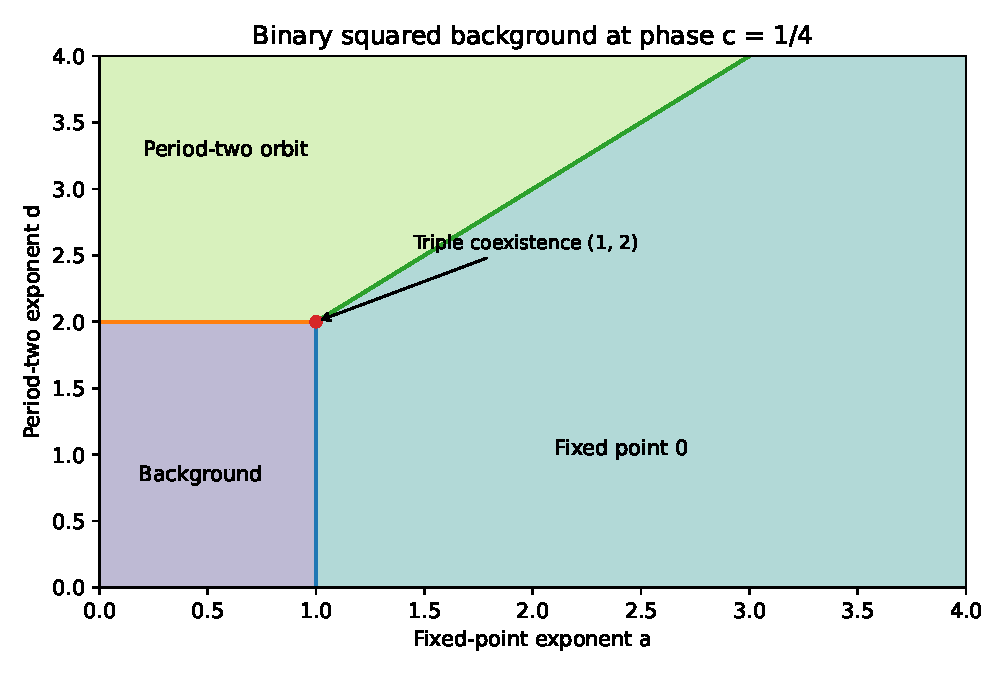
\includegraphics[width=.86\textwidth]{figures/phase_diagram.pdf}
 \caption{The mixed-moment exponent in \cref{eq:triple-moment}.
 The three affine branches meet at $(1,2)$. This is an exact phase
 diagram; the plot is only its visualization.}
 \label{fig:phase}
\end{figure}

In the general vector of exponents, the background pressure branch has
gradient $-B(r_1,\ldots,r_m)$ and orbit branch $j$ has gradient
$B(e_j-(r_1,\ldots,r_m))$. These differ. A path crossing an active
boundary transversely therefore has a first-derivative jump. A path
tangent to the boundary need not exhibit that jump in its restriction.

\section{Leading asymptotics without a background}
\label{sec:amplitudes}
Pressure determines a logarithmic growth rate, not its amplitude.
For the pure anchored product define
\begin{equation}
 J_n(\boldsymbol a)=\int_0^1
         \prod_i\prod_{p\in\cO_i}|S_{n,p}(x)|^{a_i}\dd x.
 \label{eq:pure-moment}
\end{equation}
Telescoping \cref{eq:coboundary}, with the powers of $N$ from
\cref{eq:digit-factorization}, gives the exact integral
\begin{equation}
 J_n(\boldsymbol a)=\int_0^1
                \frac{\Phi_{\boldsymbol a}(Nx)}{\Phi_{\boldsymbol a}(x)}\dd x.
 \label{eq:telescoping-moment}
\end{equation}
The quotient has removable values at $E$: $T^n$ permutes each orbit,
and numerator and denominator have the same local vanishing order.
Abbreviate $\Phi=\Phi_{\boldsymbol a}$, $\bar\Phi=\int_0^1\Phi$,
$a_* =\max_i a_i$, and $L=\lcm(r_1,\ldots,r_m)$.
Recall the positive local constants $c_p$ in \cref{eq:cp}.

\begin{theorem}[Constants, logarithms, and periodic amplitudes]
\label{thm:amplitudes}
The following three alternatives hold.

\textup{(i)} If $a_*<1$, then
\begin{equation}
 J_n\longrightarrow\bar\Phi\int_0^1\Phi(x)^{-1}\dd x.
 \label{eq:subcritical-amplitude}
\end{equation}

\textup{(ii)} If $a_*=1$, then
\begin{equation}
 J_n=2\bar\Phi\left(\sum_{p\in E:\,a(p)=1}\frac1{c_p}\right)
                      \log N+O(1).
 \label{eq:critical-amplitude}
\end{equation}

\textup{(iii)} If $a_*>1$, then
\begin{equation}
 J_n=N^{a_*-1}\bigl(C_{n\bmod L}+o(1)\bigr),
 \label{eq:supercritical-amplitude}
\end{equation}
where the positive, finite constants are
\begin{equation}
 C_r=\sum_{p\in E:\,a(p)=a_*}\frac1{c_p}
       \int_{\RR}\frac{\Phi(T^rp+u)}{|u|^{a_*}}\dd u,
       \qquad 0\le r<L.
 \label{eq:periodic-constants}
\end{equation}
The actual period can be a proper divisor of $L$.
\end{theorem}
\begin{proof}
Choose pairwise disjoint fixed neighborhoods of the points of $E$.
Near $p\in\cO_i$,
$\Phi(p+y)=c_p|y|^{a_i}(1+O(|y|))$. Constants can be chosen uniformly
over the finite set of points.

For (i), $\Phi^{-1}\in L^1(\TT)$. If $f$ is continuous and periodic
and $g\in L^1(\TT)$, then
\[
 \int_0^1 f(Nx)g(x)\dd x\longrightarrow
       \left(\int_0^1f\right)\left(\int_0^1g\right)
       \quad(N\to\infty\hbox{ through integers}).
\]
To see this, approximate $f$ uniformly by trigonometric polynomials;
for each nonconstant frequency use the vanishing at infinity of the
Fourier coefficients of $g$, which itself follows by $L^1$
approximation by trigonometric polynomials. Taking $f=\Phi$ and
$g=\Phi^{-1}$ proves the claim.

For (ii), neighborhoods of points with $a(p)<1$ and the complement of
all neighborhoods contribute $O(1)$. At a point with exponent one,
replace $\Phi(p+y)^{-1}$ by $(c_p|y|)^{-1}$. The resulting error is
$O(1)$, since the numerator is bounded. On $|y|<1/N$ the original
integral is $O(1)$ as well: its numerator is
$\Phi(T^np+Ny)=O(|Ny|)$, uniformly in the finitely many images of $p$.
For $1/N<y<\delta$, change variables $u=Ny$ to obtain
\[
 \int_1^{N\delta}\frac{\Phi(T^np+u)}u\dd u
          =\bar\Phi\log N+O(1).
\]
Indeed the periodic function $\Phi(q+u)-\bar\Phi$ has a bounded
primitive, uniformly in $q$, and integration by parts bounds its
integral against $1/u$. The negative side supplies the same leading
term. Sum over the exponent-one points.

For (iii), restrict first to a subsequence with $n\equiv r\pmod L$.
At a point with exponent $a_*$ set $y=u/N$ and divide its contribution
by $N^{a_*-1}$. The integrand converges to
$\Phi(T^rp+u)/(c_p|u|^{a_*})$. For $|u|\le1$ the numerator vanishes
to order $a_*$, so the quotient is bounded. For $|u|>1$ it is bounded
by a constant times $|u|^{-a_*}$, an integrable function. The local
denominator estimate gives these bounds uniformly on $|u|<N\delta$.
Dominated convergence proves the stated contribution.

A point of smaller exponent $a_i$ contributes at most
$O(1+\log N+N^{\max\{a_i-1,0\}})$ by splitting at $1/N$ and using
boundedness outside the inner interval. This is negligible compared
with $N^{a_*-1}$. The complement contributes $O(1)$. There are only
finitely many residue classes, so the individual subsequential limits
give \cref{eq:supercritical-amplitude}. Each limiting integral is
finite by the bounds just given and is positive because $\Phi$ is
positive off a finite set.
\end{proof}

For a single anchor $0$ with exponent one, $\bar\Phi=2/\pi$ and
$c_0=\pi$, giving the familiar coefficient $4/\pi^2$ of $\log N$.
For exponent two the limiting coefficient is one, also consistent
with the exact Parseval identity $J_n=N$. These one-anchor
normalizations are consistency checks, not new claims about classical
Dirichlet moments. The distinction specific to multiple periodic
anchors is that the constants in \cref{eq:periodic-constants} can
really differ.

\section{A uniform multivariate critical window}
\label{sec:crossover}
The logarithm at exponent one is a transition between an integrable
singularity and concentration near an orbit. Several orbits can enter
this window independently, and their leading contributions add rather
than select a single maximum.

Fix a nonempty set $C$ of orbit indices. Choose baseline exponents
$a_i^0=1$ for $i\in C$ and $0<a_i^0<1$ for $i\notin C$. For bounded
real parameters $u_i$, $i\in C$, define
\begin{equation}
 a_i(N)=1+\frac{u_i}{\log N}\quad(i\in C),
 \qquad a_i(N)=a_i^0\quad(i\notin C).
 \label{eq:critical-window}
\end{equation}
These exponents are positive for all sufficiently large $N$.
Let $\Phi_0=\Phi_{\boldsymbol a^0}$, let $c_p^0$ be its local
constants, and set
\begin{equation}
 K_i=\sum_{p\in\cO_i}\frac1{c_p^0},\qquad
 \Psi(u)=\begin{cases}(\ee^u-1)/u,&u\ne0,\\1,&u=0.\end{cases}
 \label{eq:critical-data}
\end{equation}

\begin{theorem}[Critical-window crossover]
\label{thm:crossover}
For every fixed $R<\infty$, uniformly for $|u_i|\le R$,
\begin{equation}
 J_n(\boldsymbol a(N))
 =2\left(\int_0^1\Phi_0\right)\log N
       \sum_{i\in C}K_i\Psi(u_i)+O_R(1).
 \label{eq:critical-crossover}
\end{equation}
\end{theorem}
\begin{proof}
Write $\Phi_N=\Phi_{\boldsymbol a(N)}$ and
$\bar\Phi_N=\int_0^1\Phi_N$. On compact positive exponent intervals,
$t^\alpha|\log t|$ is bounded for $0\le t\le1$. Differentiating each
factor with respect to its exponent, or integrating this bound, shows
\[
 \norm{\Phi_N-\Phi_0}_\infty=O_R((\log N)^{-1}),\quad
 \bar\Phi_N=\bar\Phi_0+O_R((\log N)^{-1}).
\]
The explicit formula for $c_p$ likewise gives
$c_p(N)=c_p^0+O_R((\log N)^{-1})$, uniformly over $p\in E$.
Local expansions of $\Phi_N$ and their relative $O(|y|)$ errors are
uniform because the exponents stay in a compact positive interval.

Points not on a critical orbit, and the complement of all fixed
neighborhoods, contribute $O_R(1)$, as their denominator exponents stay
strictly below one. Near a critical point write
$a=1+u/\log N$. Replacing the denominator by $c_p(N)|y|^a$
changes the integral by $O_R(1)$: the error is bounded by a constant
times $|y|^{1-a}$, which is uniformly integrable. On $|y|<1/N$ the
numerator vanishes to the same order $a$, and this inner contribution
is $O_R(N^{a-1})=O_R(1)$.

On the positive outer interval $[1/N,\delta]$, replace
$\Phi_N(T^np+Ny)$ by its mean. The zero-mean remainder, considered as
a function of $y$, has a primitive bounded by $C_R/N$. Integration
by parts against $y^{-a}$ bounds its contribution by
$O_R(N^{a-1})=O_R(1)$. The remaining elementary integral is
\begin{equation}
 \int_{1/N}^{\delta}y^{-1-u/\log N}\dd y
       =\log N\,\Psi(u)+O_R(1).
 \label{eq:window-integral}
\end{equation}
For $u\ne0$ this follows by evaluating the antiderivative; the result
extends uniformly across $u=0$, either by Taylor expansion or by
integrating $\ee^{ut}$ on $0\le t\le1$.
The negative interval gives the same leading term. Replacing
$\bar\Phi_N/c_p(N)$ by $\bar\Phi_0/c_p^0$ changes a term of size
$O_R(\log N)$ by only $O_R(1)$. Summing the two sides of every
critical point proves \cref{eq:critical-crossover}.
\end{proof}
At $u_i=0$, \cref{eq:critical-crossover} reduces to
\cref{eq:critical-amplitude}. The scale is $1/\log N=1/(n\log b)$
in the exponents. This result concerns pure anchored products; a
squared nontrivial background at a phase boundary may have a different
prefactor mechanism.

\section{An exact seventh-root moment with three amplitudes}
\label{sec:seventh}
The residue-class dependence in \cref{thm:amplitudes} cannot in general
be removed. The orbit $\{1/7,2/7,4/7\}$ under doubling gives a small
example that is exactly solvable at every depth.

\begin{theorem}[Exact period-three moment]
\label{thm:seventh}
For $N=2^n$ and every integer $n\ge0$,
\begin{equation}
 \boxed{\quad
 \int_0^1|S_{n,1/7}(x)S_{n,2/7}(x)S_{n,4/7}(x)|^2\dd x
 =\begin{cases}
       3N-2,&n\equiv0\pmod3,\\
       4N-2,&n\equiv1\pmod3,\\
       4N+4,&n\equiv2\pmod3.
   \end{cases}
 \quad}
 \label{eq:seventh-exact}
\end{equation}
In particular, the moment divided by $N$ has residue-class
limits $3,4,4$, and does not converge.
\end{theorem}
\begin{proof}
Let $\zeta=\ee^{2\pi i/7}$ and $\eta=\zeta+\zeta^2+\zeta^4$.
The complementary root sum is $\bar\eta=\zeta^3+\zeta^5+\zeta^6$,
and direct multiplication gives
\begin{equation}
 \eta+\bar\eta=-1,\qquad \eta\bar\eta=2,
 \qquad \eta^2+\eta+2=0.
 \label{eq:eta-relations}
\end{equation}
Indeed the product of the two sums has three terms equal to one and
each of the six nontrivial seventh roots once, giving $3-1=2$.
Define
\begin{equation}
 R(z)=\prod_{p\in\{1,2,4\}}(z-\zeta^p)
          =z^3-\eta z^2+\bar\eta z-1.
 \label{eq:R}
\end{equation}
Squaring permutes its roots, so $R(z)$ divides $R(z^N)$ for
$N=2^n$. Since
$\Phi(x)=4^{-3}|R(\ee^{2\pi ix})|^2$ for the exponent-two orbit,
\cref{eq:telescoping-moment} and Parseval identify the desired moment
with the squared coefficient norm of the polynomial $R(z^N)/R(z)$.

Let $\bar R$ mean coefficientwise conjugation. The six nontrivial
seventh roots give
\[
 R(z)\bar R(z)=1+z+\cdots+z^6,
 \qquad \frac1{R(z)}=\frac{(1-z)\bar R(z)}{1-z^7}.
\]
Thus, as a formal power series, $1/R(z)=\sum_{k\ge0}h_kz^k$ with
period-seven coefficient sequence
\begin{equation}
 (h_0,\ldots,h_6)=(-1,-\bar\eta,1,-\eta,-1,0,0).
 \label{eq:h-period}
\end{equation}
For $0\le k<N$, the coefficients in the three consecutive length-$N$
blocks of $R(z^N)/R(z)$ are
\begin{align}
 &-h_k,\notag\\
 &-h_{k+N}+\bar\eta h_k,\notag\\
 &-h_{k+2N}+\bar\eta h_{k+N}-\eta h_k.
 \label{eq:three-blocks}
\end{align}
The final two entries are zero because the quotient has degree
$3N-3$; no coefficient after these blocks is nonzero. This includes
$N=1$, where the quotient is simply one.

For $r\in\{1,2,4\}$ let $F_r(k)$ be the sum of the three squared
absolute values in \cref{eq:three-blocks}, replacing shifts by $N$
with shifts by $r$ and reading subscripts modulo seven. Using
\begin{equation}
 |x+y\eta|^2=x^2-xy+2y^2\qquad(x,y\in\ZZ),
 \label{eq:eta-norm}
\end{equation}
one obtains the following finite table entirely in integer arithmetic:
\begin{center}
\begin{tabular}{@{}c*{7}{r}r@{}}
\toprule
$r$ & $F_r(0)$ & $F_r(1)$ & $F_r(2)$ & $F_r(3)$ & $F_r(4)$ & $F_r(5)$ & $F_r(6)$ & Sum\\
\midrule
1 & 1&5&4&4&5&1&1&21\\
2 & 3&3&4&8&4&3&3&28\\
4 & 7&7&3&3&2&3&3&28\\
\bottomrule
\end{tabular}
\end{center}
By Parseval, the moment is $\sum_{k=0}^{N-1}F_r(k)$, where
$r=N\bmod7$. Write $N=7q+r$. For $r=1$, this sum is
$21q+1=3N-2$; for $r=2$, it is $28q+6=4N-2$; for $r=4$, it is
$28q+20=4N+4$. Finally $2^n\bmod7$ cycles through $1,2,4$ according
to $n\bmod3$, which proves \cref{eq:seventh-exact}.
\end{proof}

\begin{figure}[htbp]
 \centering
 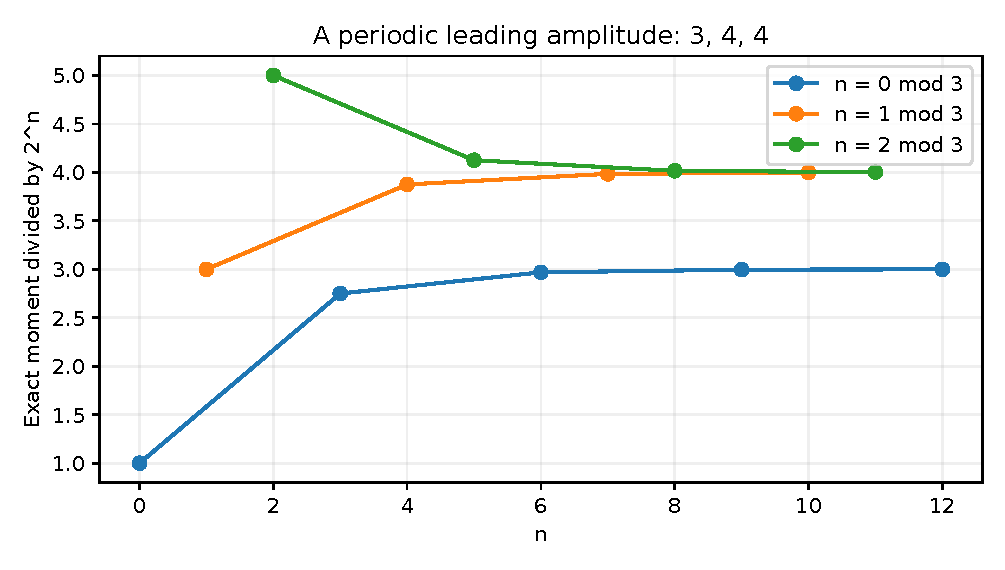
\includegraphics[width=.85\textwidth]{figures/periodic_amplitude.pdf}
 \caption{The exact seventh-root moment divided by $2^n$.
 Its residue classes approach different limits. All plotted values
 come from the exact formula, not a numerical quadrature.}
 \label{fig:amplitude}
\end{figure}

Here $D=6$ and $a_*=2$, so \cref{cor:no-background-pressure} predicts
$\PP_2(A)=-4\log2$, and the unnormalized moment has exponent one.
That correct exponent alone cannot distinguish the three leading
amplitudes. Nor can their average replace $C_{n\bmod3}$ with a
single asymptotic equivalent.

\section{Explicit realization of finite polyhedral pressure}
\label{sec:realization}
The orbit rewards can also be used constructively. The following
result prescribes a finite maximum of affine functions by an explicit
finite product, while keeping the underlying dynamical map fixed.

\begin{theorem}[Finite trigonometric realization]
\label{thm:realization}
Fix $b\ge2$, a nonempty compact set $K\subset\RR^d$, and real affine
functions $\ell_1,\ldots,\ell_m$ on $\RR^d$. Choose $m$ distinct
periodic orbits $\cO_i$ of $T_b$. There exist affine functions $c$ and
$a_i$, with $a_i(t)>0$ for all $t\in K$, such that
\begin{equation}
 w_t(x)=\ee^{c(t)}\prod_i\prod_{p\in\cO_i}m_b(x-p)^{a_i(t)}
 \quad\hbox{satisfies}\quad
 \PP_b(w_t)=\max_i\ell_i(t)\quad(t\in K).
 \label{eq:realization}
\end{equation}
The equilibrium measures are exactly the convex combinations of
$\delta_i$ for which $\ell_i(t)=\max_j\ell_j(t)$.
For each prescribed finite integer $k\ge0$, the construction can be
made $C^k$ in $x$, uniformly over $t\in K$.
\end{theorem}
\begin{proof}
Choose a constant $\ell_*<\min_{i,t\in K}\ell_i(t)$, and define
\begin{equation}
 a_i(t)=1+\frac{\ell_i(t)-\ell_*}{B},\qquad
 D(t)=\sum_i r_i a_i(t),\qquad
 c(t)=\ell_*+(D(t)-1)B.
 \label{eq:realization-construction}
\end{equation}
Every $a_i(t)>1$. By \cref{cor:no-background-pressure},
\begin{align*}
 \PP_b(w_t)
 &=c(t)-D(t)B+B\max\{1,a_1(t),\ldots,a_m(t)\}\\
 &=\max\{\ell_*,\ell_1(t),\ldots,\ell_m(t)\}
  =\max_i\ell_i(t).
\end{align*}
The background branch is strictly smaller, so the equilibrium
classification follows from \cref{thm:pressure}.

There are arbitrarily many distinct periodic orbits for fixed $b$.
For example, $1/(b^r-1)$ has exact period $r$ whenever $b^r-1>1$:
a smaller period $j<r$ would require divisibility of $b^j-1$ by
$b^r-1$, which is impossible. Choosing distinct such periods suffices.

Lowering $\ell_*$ further makes every exponent larger than $k$,
uniformly on $K$. The zeros of $m_b$ are simple in absolute-value
coordinates, and $|y|^a$ is $C^k$ for $a>k$. At any coincident mask
zeros the exponents add, preserving this property. Away from zeros
the factors are smooth. Compactness of the parameter set and a
uniform positive margin above $k$ give uniform continuity and bounds
for the derivatives through order $k$.
\end{proof}

This is a concrete realization result, not an assertion of the first
pressure-flexibility theorem; see \cite{KQ}. It also does not
contradict analyticity theorems for strictly positive H\"older weights.
Our weights vanish, so their logarithms take the value $-\infty$ at
zeros. Moreover, the parameter family is not required to be of the
restricted form $\exp(t f)$ for one everywhere-finite potential $f$.
The smoothness assertion concerns $w_t$ itself, not $\log w_t$.

\section{A nonlinear expanding-map extension}
\label{sec:nonlinear}
The selection mechanism is not inherently trigonometric. Let
$F\colon\TT\to\TT$ be a $C^1$ expanding local diffeomorphism and let
$\cO_i$ be finitely many disjoint periodic orbits of lengths $r_i$.
Put
\[
 \chi_i=\frac1{r_i}\log|(F^{r_i})'(p)|>0\qquad(p\in\cO_i).
\]
Choose a continuous $H\ge0$ whose zero set is exactly
$E=\bigcup_i\cO_i$ and whose local form is
\begin{equation}
 H(p+y)=c_p|y|^{a_i}(1+o(1)),\qquad c_p>0,
        \quad p\in\cO_i,
 \label{eq:nonlinear-H}
\end{equation}
with $a_i>0$. Such $H$ exists, for example by a finite product of
powers of distances with locally smooth positive factors.
The ratio $R=H\circ F/H$ on $\TT\setminus E$ extends continuously
to a nonnegative weight, with
\begin{equation}
 R(p)=|F'(p)|^{a_i}\frac{c_{F(p)}}{c_p}>0.
 \label{eq:nonlinear-R}
\end{equation}
It can vanish at points of $F^{-1}E\setminus E$.

\begin{theorem}[Lyapunov-weighted periodic selection]
\label{thm:nonlinear}
For every continuous $v\ge0$ with finite pressure and every real
constant $K_0$,
\begin{equation}
 \PP_F(\ee^{-K_0}vR)
 =-K_0+\max\left\{\PP_F(v),\ 
             \max_i\bigl(Q_i(v)+a_i\chi_i\bigr)\right\},
 \label{eq:nonlinear-pressure}
\end{equation}
where $Q_i(v)$ is the uniform orbit average of $\log v$.
The equilibrium measures are the corresponding convex combinations
of background equilibrium measures and maximizing orbit measures,
with the background included only when its branch is maximal.
\end{theorem}
\begin{proof}
Local differentiability of $F$ and \cref{eq:nonlinear-H} give
\cref{eq:nonlinear-R}, and hence continuity at every zero of $H$.
Away from $E$ continuity is immediate, so $R$ is bounded.
For an invariant measure giving $E$ zero mass, $F^{-1}E$ also has
measure zero. After multiplying $H$ by a positive constant we may
assume $H\le1$. Then $U=-\log H$ is finite and nonnegative almost
everywhere and $U-U\circ F=\log R$ is bounded above.
The stationary cancellation lemma gives $\int\log R=0$.
On $\cO_i$, the $c_p$ factors telescope and
$\int\log R\dd\delta_i=a_i\chi_i$.

The variational argument for weights with zeros is the same monotone
approximation as in \cref{lem:variational}. Expanding circle maps
have upper semicontinuous entropy and the continuous-potential
variational principle. Decompose invariant measures into their
selected periodic components and the component avoiding $E$.
The latter branch is unchanged by $R$, while orbit $i$ gains
$a_i\chi_i>0$. The maximum and equality cases now follow exactly as
in \cref{thm:pressure}; the scalar contributes $-K_0$.
\end{proof}
Taking $F=T_b$, $H=\Phi_{\boldsymbol a}$, and $K_0=DB$ recovers the
periodic-anchor theorem. The nonlinear extension is an exact pressure
statement. We do not assert a polynomial digital-moment representation
for a general nonlinear map.

\section{Verification, dependencies, and formalization}
\label{sec:verification}
\subsection{What the executable checks establish}
The companion \code{verify.py} uses exact integer pairs $(x,y)$ to
represent $x+y\eta\in\ZZ[\eta]$. Its multiplication rule is
\[
 (x,y)(u,v)=(xu-2yv,\ xv+yu-yv),
\]
and its norm is \cref{eq:eta-norm}. The script recomputes the entire
seven-column table in the proof of \cref{thm:seventh}. It also performs
independent exact polynomial divisions of $R(z^{2^n})$ by $R(z)$ for
$n=0,\ldots,12$, checks zero remainders, and compares the squared
coefficient norms with \cref{eq:seventh-exact}. The largest checked
$N$ is $4096$. All exact assertions passed. These finite checks are
valuable implementation tests; the all-$n$ proof is the periodic
coefficient argument, not extrapolation from the checks.

Separate floating-point diagnostics test the orbit coboundary in
bases two and three and its average on additional periodic orbits.
The mixed-moment diagnostic uses a midpoint grid with $64N$ samples
at depths $n=6,8,10,12$. For the two-anchor example at $c=1/4$, its
last two depths give the following effective exponents:
\begin{center}
\begin{tabular}{@{}rrrr@{}}
\toprule
$a$ & $d$ & Proved exponent & Effective exponent, $n=10$ to $12$\\
\midrule
0.4 & 0.7 & 1 & 1.001264\\
3.0 & 0.5 & 3 & 3.000860\\
0.3 & 4.0 & 3 & 3.002809\\
1.0 & 2.0 & 1 & 1.134007\\
\bottomrule
\end{tabular}
\end{center}
Here the effective exponent is
$(\log I_{12}-\log I_{10})/(2\log2)$ using the computed moments.
The last row is the triple point and converges much more slowly in
these finite-depth diagnostics. The exact exponent theorem permits
subpower corrections, including logarithms; we do not interpret that
row as a proven logarithmic asymptotic for the mixed family. The
critical-window computation is likewise only a diagnostic of the
bounded remainder asserted by \cref{thm:crossover}.

The full numerical data are retained in
\path{verification_results.json}. The execution summary is in
\path{verification_run.txt}.
The numerical integrations are not rigorous interval enclosures.
The script does not certify an infinite-dimensional spectrum, and none
of the proofs relies on a collocation eigenvalue.

\subsection{Proof-dependency audit}
\begin{center}
\begin{tabular}{@{}>{\raggedright\arraybackslash}p{.28\textwidth}>{\raggedright\arraybackslash}p{.66\textwidth}@{}}
\toprule
Result & Necessary ingredients\\
\midrule
Exact pressure and equilibrium faces & Continuous-potential variational
principle; upper semicontinuity and affinity of entropy; monotone
approximation at zeros; one-sided stationary cancellation; orbit
permutation.\\[1.5mm]
Global mixed-moment exponent & The pressure theorem; finite digit
factorization; Parseval; the subharmonic sampling lemma.\\[1.5mm]
Pure leading amplitudes & Exact telescoping; local vanishing orders;
periodic averaging; bounded primitives; dominated convergence.\\[1.5mm]
Critical-window formula & Uniform local expansions; an elementary
power integral; the same bounded-primitive averaging argument.\\[1.5mm]
Seventh-root exact formula & A quadratic integer ring; a cubic
polynomial; seven-periodic reciprocal coefficients; Parseval.\\[1.5mm]
Polyhedral realization & Affine normalization of the exact pressure
formula; local regularity of absolute powers.\\[1.5mm]
Nonlinear selection & Local differentiation at cycles and the same
stationary and variational arguments.\\
\bottomrule
\end{tabular}
\end{center}
No unreviewed critical-pressure asymptotic from ProveIt is an assumption
of these results. Conversely, this article does not formally certify
those neighboring manuscripts.

\subsection{A realistic Lean decomposition}
The finite algebra is a natural first tranche. Formalize the digit
factorization, the permutation of a finite periodic orbit, the
polynomial divisibility $R\mid R(z^{2^n})$, and the norm computation
in $\ZZ[\eta]$. The exact seventh-root theorem can be split into a
finite algebra lemma and a finite Fourier orthogonality statement.
This route does not need thermodynamic formalism.

For the pressure theorem, formalize the stationary cancellation lemma
with truncations first. Its only analytic inputs are invariance of the
integral and monotone convergence. Next prove the invariant-measure
energy formula, finite invariant decompositions, and the abstract
maximum-of-branches lemma. One may initially state the latter for
variational pressure, keeping the topological-pressure interface as a
separate obligation. The final interface requires the expanding-map
entropy facts and the zero-weight approximation.

Sampling and critical-window estimates form a later analytic tranche.
They need subharmonic mean inequalities, approximation in $L^1$,
local domination, and quantified uniform remainders. No Lean source is
claimed or included in the present package. The theorem decomposition
is a roadmap, not an assertion that these formal obligations have
already been discharged.

\section{Further research questions and concrete targets}
\label{sec:questions}
The following questions are deliberately narrower than asking for a
general theory of all singular phase potentials. Each has a specific
model, a diagnostic, or a proof interface supplied by this article.

\begin{question}[Breaking orbit balance]
What replaces the exact maximum law when the anchor phases cease to
form complete cycles, or exponents within a cycle become unequal?
\end{question}
A first target is the two-anchor family of \cref{sec:example}: displace
one of $1/3,2/3$ independently near $(a,d,c)=(1,2,1/4)$. Determine
whether the three-branch corner persists, rounds, or splits, and find
its leading local normal form and equilibrium selection. The exact
balanced formula supplies the limiting branches but does not control
the perturbation. The single-phase results in the repository do not by
themselves settle this mixed perturbation.

\begin{question}[Mixed critical prefactors]
At a boundary $a_iB+Q_i(c)=0$, what is the asymptotic equivalent of the
squared-background mixed moment after removing its proved power of $N$?
\end{question}
The explicit triple point $c=1/4$, $a=1$, $d=2$ is a useful benchmark.
Prove whether a logarithm, a higher power of a logarithm, a periodic
amplitude, or a different subpower correction occurs. The finite-depth
row in \cref{sec:verification} is evidence only of slow approach, not
a diagnosis. The pure-background-free theorem cannot simply be applied
because the squared background introduces a new depth-dependent
factor.

\begin{question}[When do the residue-class constants coincide?]
Characterize orbit sets and exponents for which all $C_r$ in
\cref{eq:periodic-constants} are equal.
\end{question}
The seventh-root example proves that equality is not automatic even
for a single orbit and one even exponent. Spatial symmetries can force
equality by transporting both the local constants and the integrals;
determine useful necessary conditions and classify small periods.
For even integer exponents, exact algebraic coefficient methods can
provide a finite test in examples where the corresponding rational
function is manageable.

\begin{question}[An algorithm for cyclotomic moment formulas]
For finite rational periodic phase sets with positive even integer
exponents, can every pure moment be expressed as a finite sum of powers
of $N$ with coefficients periodic in the depth?
\end{question}
The reciprocal of a polynomial with roots of unity has coefficients
which are polynomial in the coefficient index on residue classes,
with degree controlled by root multiplicity. Combine this fact with
the divisible numerator at $N=b^n$, then sum squared coefficients on
blocks. A full algorithm needs a proof of its block decomposition,
its period, and its complexity; the cubic seventh-root computation is
a small verified prototype rather than that general theorem.

\begin{question}[Infinitely many periodic anchors]
Under which summability and separation conditions does a countable
product of anchor weights define a nontrivial continuous weight, and
does its pressure admit a corresponding supremum-of-orbit formula?
\end{question}
Finite truncations give exact formulas, but an infinite product can
collapse to zero, and dense zeros can make continuity fatal to a
nontrivial limit. Control uniform convergence, the singular transfer
function, and escape of equilibrium mass before passing to a limit.
These are genuine additional issues, not formal substitutions of a
supremum for a maximum.

\begin{question}[Other background orders]
Can the anchored reduction help determine moment exponents for a
background $m_b(\cdot-c)^s$ beyond the exactly solved square?
\end{question}
The pressure theorem already reduces the answer to one single-phase
quantity $\PP_b(m_b(\cdot-c)^s)$ and finitely many orbit averages.
Insert a separately justified formula in any regime where one is
available. In particular, repository asymptotics can be combined with
this theorem after their precise hypotheses and proof status are
checked. A global exact expression for the single-phase background is
not supplied here.

\begin{question}[Positive regularization and selection at coexistence]
For $w_\varepsilon=w+\varepsilon$, determine the rate at which the
smooth positive-weight pressure approaches an anchored corner and the
limiting proportions of its equilibrium measures.
\end{question}
The proof of \cref{lem:variational} already gives monotone pressure
convergence, but neither a rate nor a selected mixture. Competing
periodic components and the background have different neighborhoods
of zeros. An analysis of these neighborhoods could produce a
finite-dimensional crossover law, but the exact maximum alone does
not identify it.

\begin{question}[Certified analysis and formal proof]
What is the smallest reusable formal interface that verifies the
pressure reduction, and can the noninteger constants $C_r$ be enclosed
rigorously and efficiently?
\end{question}
For formal proof, separate invariant-measure optimization from the
entropy and coding interface as in \cref{sec:verification}. For
numerical certification, split each integral for $C_r$ into a small
removable-singularity interval, a compact middle region, and tails
bounded by $|u|^{-a_*}$. Interval arithmetic on the compact region,
with proven local and tail bounds, would turn the current diagnostics
into certificates for concrete noninteger examples.

\section{Conclusion}
Complete periodic cycles make a mixed digital-product family exactly
tractable. The singular coboundary does not change all invariant
energies equally: it leaves an explicit periodic reward after the
common shift. This distinction gives the global pressure formula and
its full equilibrium faces. Parseval for a squared background and a
real-exponent sampling estimate then produce explicit mixed-moment
growth exponents, including exact phase boundaries and coexistence.

The leading asymptotic problem contains additional information. Without
a background it has three regimes: a finite averaging constant, a
critical logarithm, and periodic supercritical amplitudes. The
seventh-root formula shows that the arithmetic oscillation is real,
not a defect of a proof technique. The critical-window theorem and the
finite pressure-realization construction provide further concrete
consequences of the same mechanism.

These results solve the stated structured mixed problems. They do not
settle global regularity for arbitrary phase tuples, establish a
universal mixed critical prefactor, or constitute a Lean verification.
Their strongest claims are the precise formulas and proofs above;
independent review and a broader priority search remain appropriate
before describing them as an established breakthrough.

\clearpage
\begin{thebibliography}{9}
\bibitem{Walters}
P. Walters, \emph{A variational principle for the pressure of continuous
transformations}, American Journal of Mathematics \textbf{97} (1975),
937--971. DOI: \url{https://doi.org/10.2307/2373682}.

\bibitem{GKS}
P. Gohlke, M. Kesseb\"ohmer, and T. I. Schindler,
\emph{Generalized Thue--Morse measures: spectral and fractal analysis},
arXiv:2509.22109 (2025).
\url{https://arxiv.org/abs/2509.22109}.
The inspected version was the version-one HTML manuscript.

\bibitem{GLS}
P. Gohlke, G. Lamprinakis, and J. Schmeling,
\emph{On a family of singular potentials: Parameter dependence of
thermodynamic characteristics}, arXiv:2603.19001 (2026).
\url{https://arxiv.org/abs/2603.19001}.
The inspected version was the version-one HTML manuscript.

\bibitem{KQ}
T. Kucherenko and A. Quas, \emph{Flexibility of the pressure function},
Communications in Mathematical Physics \textbf{395} (2022), 1431--1461.
DOI: \url{https://doi.org/10.1007/s00220-022-04466-y}.
Preprint: \url{https://arxiv.org/abs/2108.00451}.

\bibitem{Repo}
V. Reshetnikov and contributors, \emph{ProveIt}, research and
formalization repository. Snapshot inspected on 30 September 2026:
\nolinkurl{781594d886f8dc56069221e2b56bd1e94d9c6e5f}.
\url{https://github.com/VladimirReshetnikov/ProveIt/tree/781594d886f8dc56069221e2b56bd1e94d9c6e5f}.

\bibitem{RepoIndex}
\emph{Thue--Morse research index}, in \cite{Repo}, path
\path{Analysis/FabiusFunction/docs/semi-formalized-research-frontiers/drafts/thue-morse/README.md}.
Inspected together with the critical and subcritical pressure
manuscripts. The index records integer, fractional, critical,
subcritical, and critical-correction arrivals and labels those recent
reports unreviewed, with no Lean statement. This is provenance and
scope information, not a mathematical hypothesis of the present article.
\end{thebibliography}
\end{document}
